\documentclass[border=10pt]{standalone}
\usepackage{tikz}
\usetikzlibrary{arrows.meta, circuits.ee.IEC, calc, positioning}
\tikzset{
  >=Stealth,
  component/.style={draw, line width=0.8pt},
  lab/.style={font=\small},
}

\begin{document}
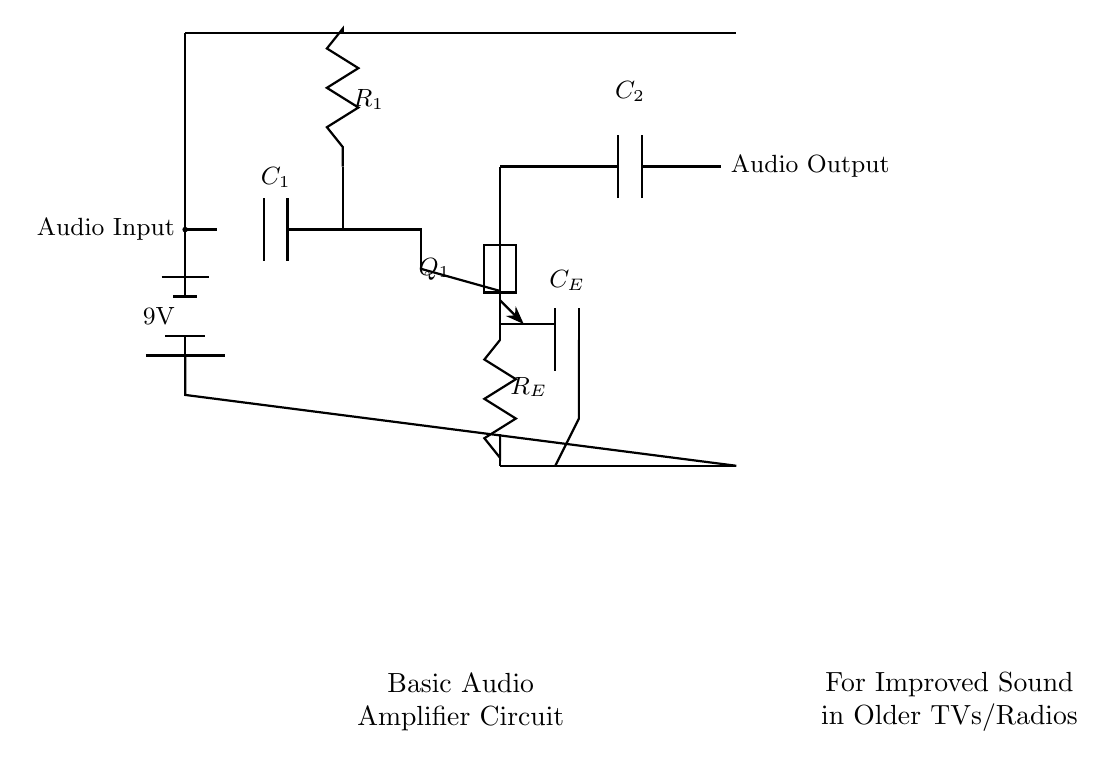
\begin{tikzpicture}[circuit ee IEC, line width=0.8pt]

% coordinates for main rails
\coordinate (leftmid) at (0,0);
\coordinate (topL)    at (0,2.5);
\coordinate (botL)    at (0,-3);
\coordinate (topR)    at (7,2.5);
\coordinate (botR)    at (7,-3);

% Vertical main wire (mid) from top to bottom
\draw (topL) -- (0,1.2); % down to above input node

% Audio Input node
\draw (leftmid) node[lab, left]{Audio Input} -- (0,0); % small extension
\coordinate (inputnode) at (0,0);

% continue vertical wire down to battery top node
\draw (0,1.2) -- (inputnode) -- (0,-0.6);

% Battery 9V
\coordinate (batTop) at (0,-0.6);
\coordinate (batBot) at (0,-1.6);
\draw (batTop) ++(-0.3,0) -- ++(0.6,0);
\draw (batTop) ++(-0.15,-0.25) -- ++(0.3,0);
\draw (batBot) ++(-0.5,0) -- ++(1.0,0);
\draw (batBot) ++(-0.25,0.25) -- ++(0.5,0);
\draw (batTop) -- ++(0,-0.25);
\draw (batBot) -- ++(0,0.25);
\node[lab,left] at ($(batTop)!0.5!(batBot)$) {9V};

% Bottom rail
\coordinate (bot) at (0,-2.1);
\draw (0,-1.6) -- (bot) -- (botR);

% Top rail
\draw (topL) -- (topR);

% C1 between input node and base node
\coordinate (C1R) at (2,0);
\draw (inputnode) -- ++(0.4,0);
\draw (1,0.4) -- (1,-0.4); % left plate
\draw (1.3,0.4) -- (1.3,-0.4); % right plate
\draw (1.3,0) -- (C1R);
\node[lab, above] at (1.15,0.4) {$C_1$};

% R1 from top rail down to base node (C1R)
\draw (C1R) -- ++(0,0.8);
\coordinate (R1bot) at (2,0.8);
\coordinate (R1top) at (2,2.5);
% resistor zigzag
\draw (R1bot) -- ++(0,0.25)
  -- ++(-0.2,0.25)
  -- ++(0.4,0.25)
  -- ++(-0.4,0.25)
  -- ++(0.4,0.25)
  -- ++(-0.4,0.25)
  -- ++(0.2,0.25)
  -- (R1top);
\node[lab, right] at ($(R1top)!0.5!(R1bot)$) {$R_1$};

% Base node to transistor base
\coordinate (base) at (2,0);

% Transistor Q1 position
\coordinate (Q1) at (4,-0.5);

% Connect base node to transistor base
\draw (base) -- (3,0) -- (3,-0.5);

% Draw NPN transistor symbol manually
% Collector up
\coordinate (col) at (4,0.8);
\coordinate (emit) at (4,-1.2);
\draw (col) -- (Q1);
\draw (emit) -- (Q1);
% base line
\draw (3,-0.5) -- ($(Q1)!0.4!(emit)$);

% transistor circle omitted, just outline:
\draw ($(Q1)+(-0.2,-0.3)$) -- ($(Q1)+(0.2,-0.3)$) -- ($(Q1)+(0.2,0.3)$) -- ($(Q1)+(-0.2,0.3)$) -- cycle;

% emitter arrow
\draw[->] ($(Q1)!0.5!(emit)$) ++(0,-0.05) -- ++(0.3,-0.3);

\node[lab, left] at ($(Q1)+(-0.5,0)$) {$Q_1$};

% RE resistor from emitter node to bottom rail
\coordinate (Etop) at (emit);
\coordinate (Ebot) at (4,-3);
% connection downward from emitter
\draw (Etop) -- ++(0,-0.2);
\coordinate (ReTop) at (4,-1.4);
\coordinate (ReBot) at (4,-2.6);
% Zigzag for RE
\draw (ReTop)
  -- ++(-0.2,-0.25)
  -- ++(0.4,-0.25)
  -- ++(-0.4,-0.25)
  -- ++(0.4,-0.25)
  -- ++(-0.4,-0.25)
  -- ++(0.2,-0.25)
  -- (ReBot);
\draw (ReBot) -- (4,-3);
\draw (4,-3) -- (botR);
\node[lab, right] at ($(ReTop)!0.5!(ReBot)$) {$R_E$};

% CE capacitor from emitter node to bottom rail
\coordinate (CEleft) at (4.7,-1.4);
\coordinate (CEbot)  at (4.7,-3);
\draw (Etop) -- ++(0.7,0) -- (CEleft);
\draw (CEleft) ++(0,0.4) -- ++(0,-0.8); % left plate
\draw (CEleft) ++(0.3,0.4) -- ++(0,-0.8); % right plate
\draw (CEleft) ++(0.3,0) -- ++(0,-1.0) -- (CEbot);
\node[lab, above] at ($(CEleft)+(0.15,0.5)$) {$C_E$};

% C2 coupling capacitor from collector node to output
\coordinate (C2L) at (5.5,0.8);
\coordinate (C2R) at (6.8,0.8);
\draw (col) -- (C2L);
\draw ($(C2L)+(0,-0.4)$) -- ++(0,0.8);  % left plate
\draw ($(C2L)+(0.3,-0.4)$) -- ++(0,0.8); % right plate
\draw ($(C2L)+(0.3,0)$) -- (C2R);
\node[lab, above] at ($(C2L)+(0.15,0.7)$) {$C_2$};
\node[lab, right] at (C2R) {Audio Output};

% Label Audio Input already added; add small dot at junction
\fill (inputnode) circle (1pt);

% Bottom captions
\node[below=2.5cm of $(botL)!0.5!(botR)$, align=center] (capL)
  {Basic Audio\\Amplifier Circuit};
\node[right=3cm of capL, align=center] (capR)
  {For Improved Sound\\in Older TVs/Radios};

\end{tikzpicture}
\end{document}